\documentclass[12pt]{article}
\usepackage{fullpage}
\usepackage[noend]{algpseudocode}
\usepackage{algorithmicx}
\usepackage{algorithm}
\usepackage{amssymb}
\usepackage{amsmath}
\usepackage{graphicx}
\newcommand{\realpositivenumbers}{\mathbb{R}_{>0}} %Real numbers symbol
\newcommand{\bigO}{\mathcal{O}}

\begin{document}

\section*{ADM (2019) - Homework 2}

\subsection*{Theoretical Question}
\vspace{.5cm}

You are given the following functions:
\vspace{.4cm}


\begin{algorithm}
\caption{splitSwap}\label{splitFun}
\begin{algorithmic}[1]
\Function{splitSwap}{a, i, n}:
\If {$i \leq 1$} 
	\State \Return 
\EndIf

\State \Call{splitSwap}{a, $i$, $n/2$}
\State \Call{splitSwap}{a, $i+n/2$, $n/2$}
\State \Call{swapSplit}{a, $i$, $n$}
\EndFunction
\end{algorithmic}
\end{algorithm}

\begin{algorithm}
\caption{swapList}\label{swapFun}
\begin{algorithmic}[1]
\Function{swapList}{a, l, n}:
\For {$i=0 \leq n/2$}
\State tmp = a[$l + i$]
\State a[$l + i$] = a[$l + i + n/2$]
\State a[$l + i + n/2$] = tmp
\EndFor
\EndFunction
\end{algorithmic}
\end{algorithm}

\begin{enumerate}
\item How much running time does it take to execute \textproc{splitSwap}(a, 0, n)? Use Big-O analysis.
\item What does this algorithm do? Is it optimal? Describe the mechanism of the algorithm in details, we do not want to know only its final result.
\end{enumerate}
\pagebreak

\subsection*{1. Solution}

Let's start by first analyzing the second function, \textproc{swapList} as it is called inside the other function we want to 
analyze. 

We can split the code into two parts: the assignments (which allow us to swap two values) and the loop.
Then we can start writing the analysis for time complexity of this function: 

$$ T_2(n) = 3\ c_1 \cdot (c_2\ (n/2))$$

This means that we suppose each of the 3 assignment to take approximately $c_1$ units of time. The loop performs a check for
each iteration, hence $c_2$.
We can already start dropping lower order terms and constants that don't help us with the analysis, so we have that:
$$ T_2(n) = n/2 $$

We can now try to find a function that allow us to define the complexity of the \textproc{splitSwap} function.
\vspace{1cm}

Let $f(n) = n $ and $g(x) = T_2(n) = n/2$. If we are able to find a $c \in \realpositivenumbers$ such that for 
any $n \geq n_0$ we have that $g(n) \leq cf(n)$, we can say that \textproc{splitSwap} is $\bigO(n)$.

We have:

$$ \frac{n}{2} \leq c\ n $$
$$ 1 \leq 2c $$
$$ c \geq \frac{1}{2} $$

Let's try to find a lower bound for our function in analysis. We choose $h(n) = n$ and $g(n) = n / 2$, and see if we find a $c \in \realpositivenumbers $ such that for each $n \geq n_0$ we have that $g(n) \geq c\ h(n)$.

$$ g(n) \geq c f(n) $$
$$ n/2 \geq c n $$
$$ c \leq \frac{1}{2} $$

We have found a constant so that $g(x) \geq \frac{1}{2}\ f(x)$ for all $n \geq n_0$, so we can say that $g(x)$ is $\Omega(n)$.
\vspace{1cm}

Since we want also to build a tighter bound for defining the complexity of $g(x)$, we can intersect the previously found sets of constants $c$ such that $c\ f(n) \geq g(n) \geq c\ h(n)$, we find that $c = \frac{1}{2}$ is the only solution.

Having found such constant, we can now say that $g(n)$ is $\theta (n)$.
\pagebreak

We can now start analyzing the complexity of \textproc{splitSwap}. Since we found that \\ \textproc{swapList} is $\theta(n)$ we 
can put it easily in the \textproc{splitSwap} recursive definition:

\begin{equation}
  T(n) =\begin{cases}
    \theta(1) & \text{if $n \leq 1$}.\\
    2T\left( \frac{n}{2} \right) + \theta(n) & \text{otherwise}
  \end{cases}
\end{equation}

The algorithm is in a \textit{divide-et-impera} recurrence form and the way such recurrence is defined might 
allow the use of the Master Theorem. Let's first see how the recurrence relation in the MT presents itself in variable form: 

\begin{equation}
	T(n) = a T\left( \frac{n}{b} \right) + f(n)
\end{equation}

Choosing $a = 2$, $b = 2$, and $f(n) = n$ we get:

\begin{equation}
	T(n) = 2 T\left( \frac{n}{2} \right) + n
\end{equation}

Which is the inductive case definition of \textproc{splitSwap} (so for $n > 1$). This algorithm is shown to be 
$\theta(n \log{n})$, in the case of $f(n) = \theta(n^{log_b{a}}) = \theta(n^{log_2{2}}) = \theta(n)$ and assuming that $n$ is 
a perfect power of $2$.
                                                                                                                                                                                                                                                                     

                                                                                                                                                                                                                                                                    It might be easier to visualize using this recursion tree representation:
                                                                                                                                                                                                                                                                    \begin{figure}[h]                                                                                                                                                                                                                                                                    \caption{Image from \textit{Introduction to Algorithms, CLRS}}                                                                                                                                                                                                                                                                     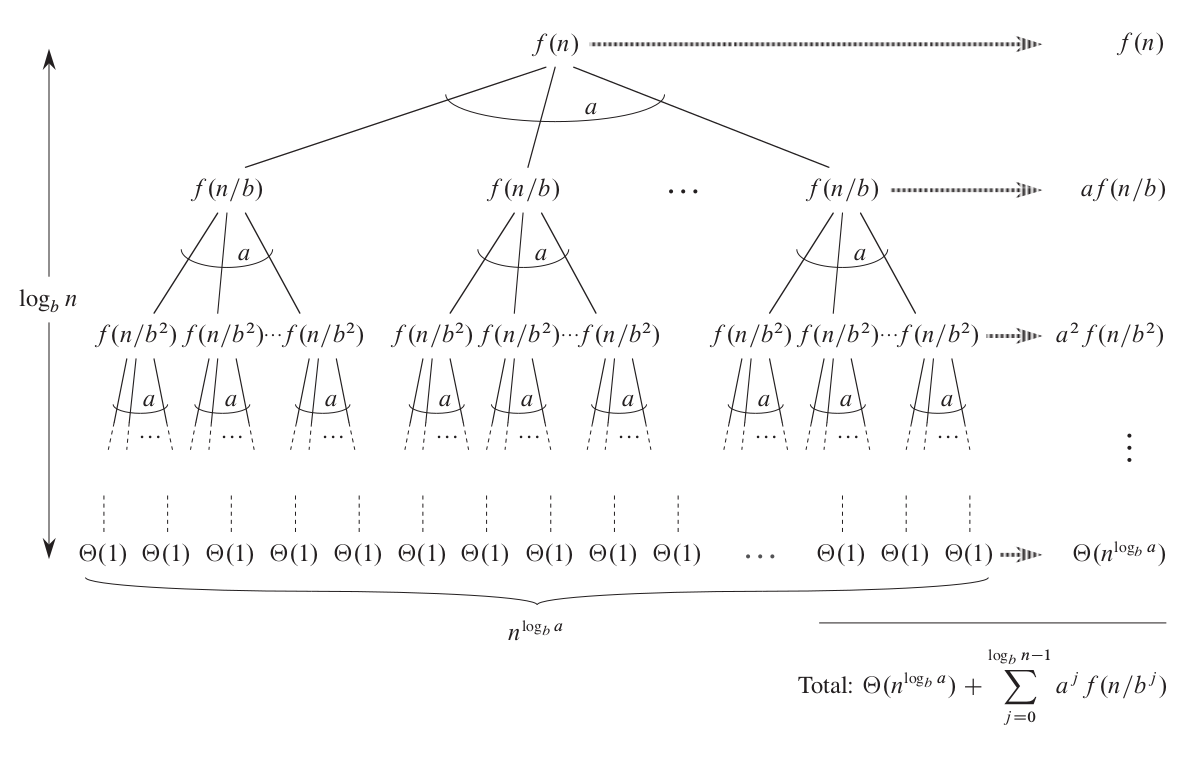
\includegraphics[scale=.4]{./recursion_tree_clrs.png}                                                                                                                                                                                                                                                                   
\centering
\end{figure}

                                                                                                                                                                                                                                                                     


\end{document}
